\section{La guilde des Voleurs}

La guilde des voleurs consiste en réalité en une alliance de divers groupes 
clandestins opérant dans et autour de la ville de Sichua. La guilde est 
localisée dans des sous terrains se trouvant sous la colline des nobles
avec des accès à la fois vers la cote, les quartiers suds et les quartiers 
plus riches directement au dessus du complexe (voir carte). La guilde est
dirigée par huit maîtres: le maître assassin, le maître comptable, le maître 
esclavagiste, le maître escroc, le maître racketteur, le maître pirate, le 
maître voleur et la grande maîtresse (sous-entendu des prostituées). Ces huits 
dirigeants sont en charge des huits activités criminelles de la guilde et
s'occupent de la coordination entre les différentes branches. Le leader
de la guilde est généralement le maître assassin, un personnage 
particulièrement mystèrieux connu seulements des autres maîtres à la
tête d'un groupe de meurtrier aussi efficaces que discrets.


\begin{figure*}[p]
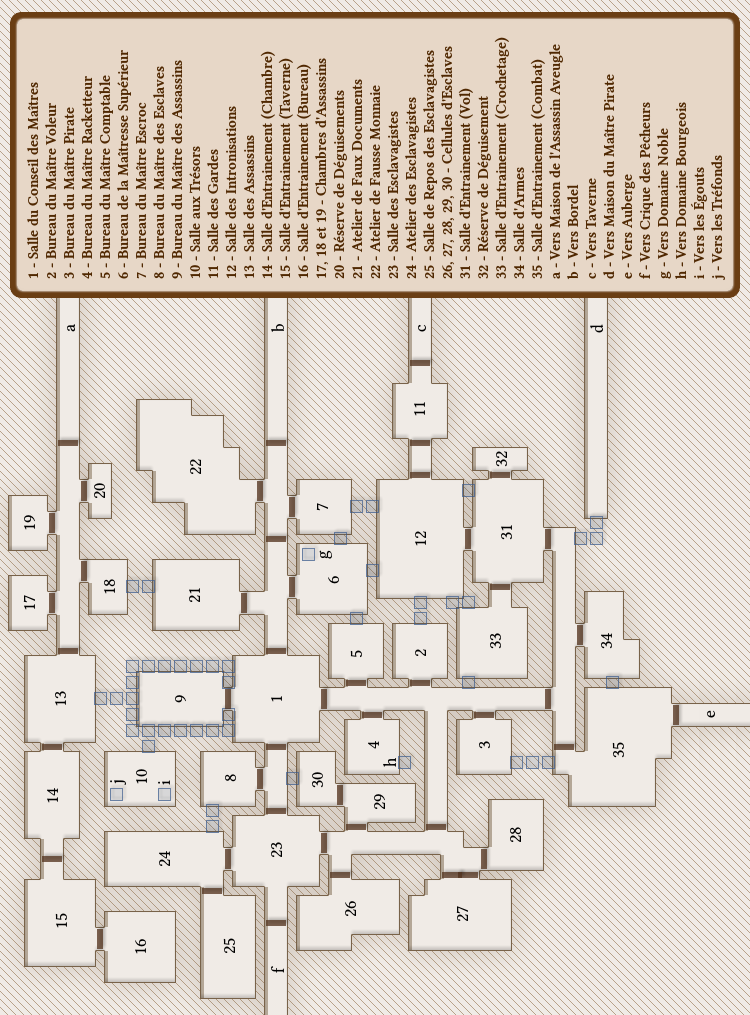
\includegraphics[width=17cm]{Maps/GuildeVoleurs.png}
\end{figure*}

\subsection{Les Groupes Locaux}

La ville de Sichua est en fait occupée en grande partie par des groupes
semi-indépendants ayant prété allégence à la guilde. Ceux-ci font appels 
à la guilde pour recevoir des renforts en cas de besoins ou de préparation 
d'un gros coup, mais doivent aussi s'aquitter d'une taxe auprès de celle-ci. Ils dépendent
d'un maître différent en fonction de leur localisation géographique:
l'ile de la source au maître assassin, le quartier des marchés au maître
comptable, le quartier du port sud au maître esclavagiste, le quartier 
bourgeois au maître escroc, le quartier pauvre du sud au maître racketteur,
le quartier du port nord au maître pirate, les quartiers nords au maître 
voleur et le quartier noble à la grande maîtresse. Cette dépendence hiérarchique 
n'empèche bien sur pas chaque groupe local de pratiquer n'importe lesquelles des huits
activités. Néanmoins, il est clair que ces groupes de petites frappes ne sont
jamais vraiment très puissant. 

Les groupes locaux ne couvrent néanmoins pas tout le territoire de la ville
et un certain nombre d'agents de la guilde dépendent directement d'un maître.
Ceux-ci sont en général les meilleurs agents des groupes locaux et sont recrutés
par la guilde pour s'occuper des affaires les plus lucratives directement. 
Les plus expérimentés obtenant finalement la direction d'un groupe local
si ils survivent suffisamment longtemps dans le milieu. Les chefs de groupe
locaux ont aussi un pouvoir important pour nominer un nouveau maître
lorsque l'ancien disparait. Ils décident alors de la promotion de l'un d'entre 
eux au rang de maître. Il est a noté qu'aucun groupe de malfrats n'est connu 
sur l'île de la source, le système de promotion du maître assassin échappe donc
à cette règle, mais reste un mystère pour le reste de la guilde.

%Liens vers groupe évoqué dans la quête ?


\subsection{Les Faussaires}

Dans le complexe de la guilde se trouvent deux ateliers important, l'un
accueillant de véritables artistes experts en conception de faux documents
et en imitations de signatures et l'autre est dédié à la fabrication de fausses 
monnaies. Le maître comptable est en charge de l'exploitation des ces deux
ateliers et de la diffusion de leurs produits. La fabrication de faux en
particulier est généralement utilisé pour des escroqueries de haut niveau
permettant souvent de voler de véritables fortunes.

Le maître comptable est un riche marchand ...

\subsection{Les Esclavagistes}

L'esclavagisme est interdit à Sichua, néanmoins il est possible d'y transferer
et d'y vendre vos esclaves si vous avez de bons contacts. Les esclavagistes 
utilisent une petite crique discrète dans le sud de Sichua pour transférer
les esclaves qui sont gardés directement dans les sous terrains de la guilde.
Ceux-ci seront exportés ensuite vers des îles loin au sud de Sichua, où la
pratique est légale. 

Le maître esclavagiste est un riche ...

\subsection{Les Escrocs}


Le maître escroc est Meribald Dalloris (page \pageref{MeribaldDalloris}).

\subsection{Les Racketteurs}


\subsection{Les Pirates}


\subsection{Les Voleurs}


\subsection{Les Prostituées}


\subsection{Les Assassins}


\subsection{Rapports à l'Exterieurs}

Un nouveau maître en charge des paris clandestins ?

Un accord secret avec les Alchimistes

Sert de source d'information à certains dirigeants

Siège au conseil des cinq
